\documentclass[12pt,fleqn,a4paper]{article}

\usepackage{latexsym}
\usepackage{url}
\usepackage{xspace}
\usepackage{epsfig}
\usepackage{psfrag}
\usepackage{a4wide}
\usepackage{marvosym}
\usepackage{amsmath,amsfonts,amssymb,amsthm,latexsym}
\usepackage{graphics,graphicx,color,subfigure}
\usepackage{fancyhdr}
\usepackage[english]{babel}
\usepackage[latin1]{inputenc}
\usepackage{algorithm}
\usepackage{algorithmic}


\textheight 680pt
\textwidth 460pt
\topmargin -40pt
\oddsidemargin 5pt
\evensidemargin 5pt
\parindent 0pt

\pagestyle{fancyplain} \setlength{\headheight}{16pt}
\renewcommand{\sectionmark}[1]{\markright{\thesection\ #1}}
\lhead[\fancyplain{}{\thepage}]
    {\fancyplain{}{\rightmark}}
\rhead[\fancyplain{}{\leftmark}]
    {\fancyplain{}{\thepage}}
\cfoot{}
\renewcommand{\thesection}{\arabic{section}}
\renewcommand{\thesubsection}{\arabic{section}.\arabic{subsection}}


\begin{document}
\begin{titlepage}%Institution
\vspace{2cm}
\centerline{
\large{Department of Artificial Intelligence and Human Interfaces}}
\vspace{0.2cm}
\centerline{\large{University of Salzburg}}%Title with one or two Lines(More if wanted)
%\hline
\vspace{1cm}

\centerline{\large{PS Natural Computation}}
\centerline{SS 24}
\vspace{1cm}

\centerline{\Large\textbf{Dynamic Optimization of Target Values}}
\vspace{0.3cm}
\centerline{\Large\textbf{in Neural Network Classification}}
\vspace{1cm}

\vspace{0.4cm}%Date
\centerline{\today}
\vspace{5cm}%Authors

%\hline
\vspace{0.2cm}
Project Members:\\
\centerline{Andrassik Leon, 12209906, leon.andrassik@stud.plus.ac.at}\\
\centerline{Bhuiyan Amreen, 12203597, amreen.bhuiyan@stud.plus.ac.at}\\
\centerline{Yakar Bet\"ul, 12205751, betuel.yakar@stud.plus.ac.at}\\
\centerline{Zauner Sofia, 12118492, sofia.zauner@stud.plus.ac.at}\\
\vspace {1cm}\\

Academic Supervisor: \\
\centerline{Helmut MAYER}
\centerline{helmut@cosy.sbg.ac.at}
\vspace{1.5cm}\\
Correspondence to: \\
\centerline{Universit\"{a}t Salzburg} \\
\centerline{Fachbereich AIHI} \\
\centerline{Jakob--Haringer--Stra\ss e 2} \\
\centerline{A--5020 Salzburg} \\
\centerline{Austria}
\clearpage
\end{titlepage}

%Table of Content
% \setcounter{page}{1}
% \pagenumbering{Roman} %I,II,III... in the TOC
% \tableofcontents

\clearpage
\pagestyle{headings}
\pagenumbering{arabic}  %Better if TOC is variable (more than one page)
\setcounter{page}{1}
\pagenumbering{arabic}  %Better if TOC is variable (more than one page)
\setcounter{page}{1}

\abstract{The aim of our project is to implement an alternative method of choosing target values for classification with neural networks.  Instead of using traditional one-hot encoding, which uses fixed values of 0 and 1, this method involves assigning custom target values to each class. 

These target values are dynamically optimized during the training process, which distinguishes our approach from conventional fixed-target training. Our idea is to capture the model's natural predictions and use these to refine the target values.

This approach requires a new rule for determining the predicted class: rather than choosing the neuron with the highest value, we select the neuron whose output value is closest to its corresponding target value and therefore has the lowest error; a method we will refer to as "minimum distance classification".

To evaluate the performance of our approach, we will employ the MNIST dataset and compare with the one-hot encoding method.}

\vspace{4em}

\section{Introduction}
Artificial neural networks (ANNs) have become essential tools in modern classification tasks, mapping complex input data to discrete predefined output categories. During training, the error is calculated as the difference between the desired output and the actual output produced by the network. The objective of the training process is to minimize this error through iterative adjustments of the network's weights and biases. Following the training phase, performance is evaluated using a test set that contains previously unseen data, providing a neutral measure of its generalizability and classification accuracy. \\

Traditionally, the learning process of such networks is based on one-hot encoded target values, where the correct class is represented by the value 1, and all others are assigned a 0. This binary approach became standard due to its simplicity and compatibility with widely used loss functions. However, enforcing these extreme target values could potentially lead to challenges depending on the system's underlying activation function. It may negatively affect gradient flow, reduce training efficiency, and encourage overconfident predictions. \\

One-hot encoding enforces a "winner-takes-all" (WTA) dynamic, where only the neuron with the highest output is considered correct. Since the target vector consists of a 1 for the correct class and a 0 everywhere else, this is effectively equivalent to selecting the output that is closest to its respective target value. Thus, WTA can be considered a special case of a more general strategy, which is known as nearest target or minimum distance classification. Here, we make a general comparison between the entire output distribution given by the network and the available target vectors for each class. Whichever class's target the output is closest to (using a distance metric such as Euclidean distance) will be chosen as the correct class. \\

In this project, we propose a more flexible approach for target value assignment in classification networks. Instead of defining fixed values of 0 and 1, we generate target vectors composed of custom class and non-class values. Here, class values refer to the target values assigned to the positions which would ordinarily be filled with 1 in a one-hot vector, while the non-class values fill all other positions. These alternative targets are not chosen arbitrarily, but rather inferred from the model's own inherent output tendencies during training. By adapting target values dynamically in response to the network's evolving behavior, we aim to guide learning in a way that is more aligned with the model's natural predictions. \\

This change calls for a rethinking of how predictions are interpreted. Rather than treating each neuron as directly representing a class, we consider the entire output vector and assign the prediction to the class whose target vector lies closest under a chosen distance metric. Our goal is to design an algorithm that leverages this strategy of dynamic target values and to evaluate its performance relative to existing approaches. 

\section{Classification with Artificial Neural Networks}\label{sec:class}
ANNs are computational models inspired by the functioning and structure of the human brain, designed to simulate the way biological neurons process information. These networks serve as a powerful tool in complex pattern recognition and play a fundamental role in solving machine learning problems.  In this section, we provide an overview of Artificial Neural Networks exploring their basic architecture and functionality, while also giving insight on their application in classification tasks.

\subsection{Structure of Artificial Neural Networks}

\begin{figure}[H]
    \centering
    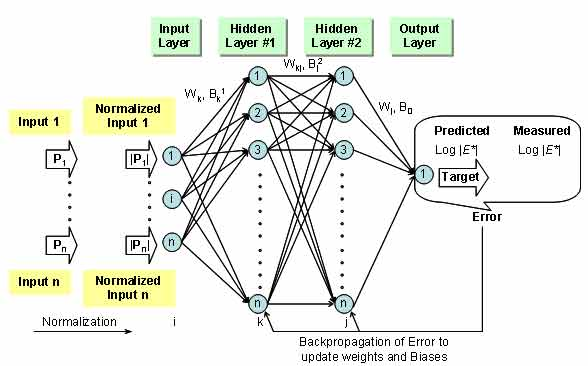
\includegraphics[width=0.56\linewidth]{graphs/annStructure.jpg}
    \caption{Network structure for training ANN models  \cite{FHWA}}
    \label{fig:annStruct}
\end{figure}

An Artificial Neural Network consists of a multitude of interconnected nodes, or neurons, organized into layers. Each layer is designed to process input data and pass the resulting output signals to the following. To achieve this, each neuron receives one or more inputs, applies respective weights and a bias, and then forwards the result through an activation function. Typically, a Neural Network is composed of three types of layers, as also visualized in Figure \ref{fig:annStruct}:

\begin{itemize}
     \item \textbf{Input Layer:} The input layer is the first layer of the network and is responsible for receiving the raw input data. Each neuron in this layer represents a specific feature of the input. For example, in an image classification task, each input neuron may correspond to a single pixel of the given image.
     \item \textbf{Hidden Layers:} The hidden layers are located between the input and output layers. Most of the actual computation takes place here. The neurons in these layers take the output of the previous layer as input, process this information, and send their output to the next layer. The number and size of the hidden layers vary depending on the complexity of the problem and the depth of the network.
     \item \textbf{Output Layer:} This concluding layer produces the network's final output. In a classification task, the output layer usually consists of one neuron per possible class, with each neuron's output representing the network's prediction for the corresponding class.
\end{itemize}

Each neuron in a layer is connected to every neuron in the previous and the following layer, creating a fully connected, dense network. These connections are defined by the weights, which are adjusted during the training process.


\subsection{Inner Workings of a Neuron}
The process by which a neuron works can be described by the following two steps:
 \begin{enumerate}
 \item \textbf{Aggregation Function:} Each neuron receives one or more input signals. Within input layers these signals correspond to raw data, whereas in the case of hidden layers they originate from the outputs of the previous layer. Among other things, the obtained data contains information on the corresponding weights and biases. The weights determine the strength of the connection between two neurons. During training the weights are adjusted accordingly, further explained in Section~\ref{sec:training_proc}. The bias is used to shift the activation function to improve the learning process. 
Now the aggregation function, which is used to calculate the weighted sum of the given inputs by multiplying each input value by its corresponding weight, adding the bias, and summing up the products, is applied. The weighted sum $z$ of a neuron can be computed as follows, where $x_i$ denotes the inputs, $w_i$ the weights, and $b$ the bias: \\
$$z_i = \sum_{i=1}^n x_i* w_i +b$$

 \item \textbf{Activation Function:} In the next step, the weighted sum $z_i$ is passed through the activation function. This function introduces non-linearity into the network, which enables the system to recognize, learn, and model complex non-linear patterns. The final output of the neuron in the layer is the result of the activation function applied to the weighted sum of its inputs. Two commonly used activation functions, which were also applied in this project (see Section~\ref{sec:net_arch}), are the sigmoid and the Softmax activation functions. They are defined as follows:
\begin{itemize}
\item \textbf{Sigmoid-activation function:} The sigmoid function maps any input to a value between 0 and 1, making it ideal for binary classification problems. 
\item[]\hspace{1.25cm}$\Rightarrow \sigma(z_i)=\frac{1}{1+e^{-z}}$

\item \textbf{Softmax-activation function:} The Softmax function converts the raw output into a probability distribution across all k classes and is therefore often used in the output layer of classification networks.
\item[]\hspace{1.25cm}$\Rightarrow Softmax(z_i)=\frac{e^{z_i}}{\sum_{j=1}^{k} e^{z_j}}$
\end{itemize}
\end{enumerate}

\subsection{Training Process}\label{sec:training_proc}
The objective of the training process in an ANN is to adjust the network's weights and biases to minimize the error between the actual output and the target values. This is achieved through a method called backpropagation. In this process the network iteratively updates its parameters using the gradients of the loss function with respect to each weight and bias in the direction that reduces the error. The loss function guides the optimization process by quantifying the difference between the expected and the generated outputs. One commonly used loss function in classification tasks is the negative Log-Likelihood loss (NLL). This function measures the difference between the network's predicted probability distribution given by the log softmax function and the target vectors. The Negative Log-Likelihood (NLL) loss is defined as:

\[
\text{NLL}(z_i) = -\sum_{j=1}^{M} y_{ij} \log \hat{y}_{ij}
\]

where:
\begin{itemize}
  \item \( y_{ij} \) is the target label for class \( j \) in one-hot encoding (1 for the correct class, 0 otherwise),
  \item \( \hat{y}_{ij} \) is the predicted probability for class \( j \),
  \item \( M \) is the total number of classes.
\end{itemize}

Since only one \( y_{ij} \) is 1 (the correct class), this simplifies to:

\[
\text{NLL}(z_i) = -\log \hat{y}_{i,c}
\]

where \( c \) is the index of the correct class for sample \( i \).

\subsection{Convolutional Neural Networks}
A Convolutional Neural Network (CNN) is a specialized type of artificial neural network designed for systems needing object detection, segmentation, and recognition, such as image classification networks. The key difference between CNNs and traditional ANNs lies in their architecture. CNNs use convolutional layers to automatically detect significant patterns at different levels of abstraction, like edges, textures, or shapes, directly from the raw input data, eliminating the need for manual feature extraction.
The architecture of a CNN typically consists of these three layer types:
\begin{itemize}
\item\textbf{Convolutional Layers:} These layers are the core components of CNNs. A convolutional layer applies filters, also known as kernels, to the input data, performing a convolution operation that extracts specific (learned) attributes. Each filter detects a different feature, like an edge or texture, in a small region of the input and generates a feature map that indicates the presence and strength of the corresponding feature within the input image. After convolution, the output is passed through an activation function, analogous to the ANN structure.

\item\textbf{Pooling Layers:} Pooling layers are typically placed after convolutional layers. They reduce the spatial dimensions of the feature maps by extracting the most important information, which also helps reduce the computational load. Common pooling methods include max pooling and average pooling.

\item\textbf{Fully Connected Layers:} After several convolutional and pooling layers, the network typically includes one or more fully connected layers. In these layers each neuron is connected to every neuron in the previous layer. They are typically used to hierarchically combine the extracted features and make the final prediction or classification.
\end{itemize}

\subsection{Classification Mechanisms}
\begin{figure}[H]
    \centering
    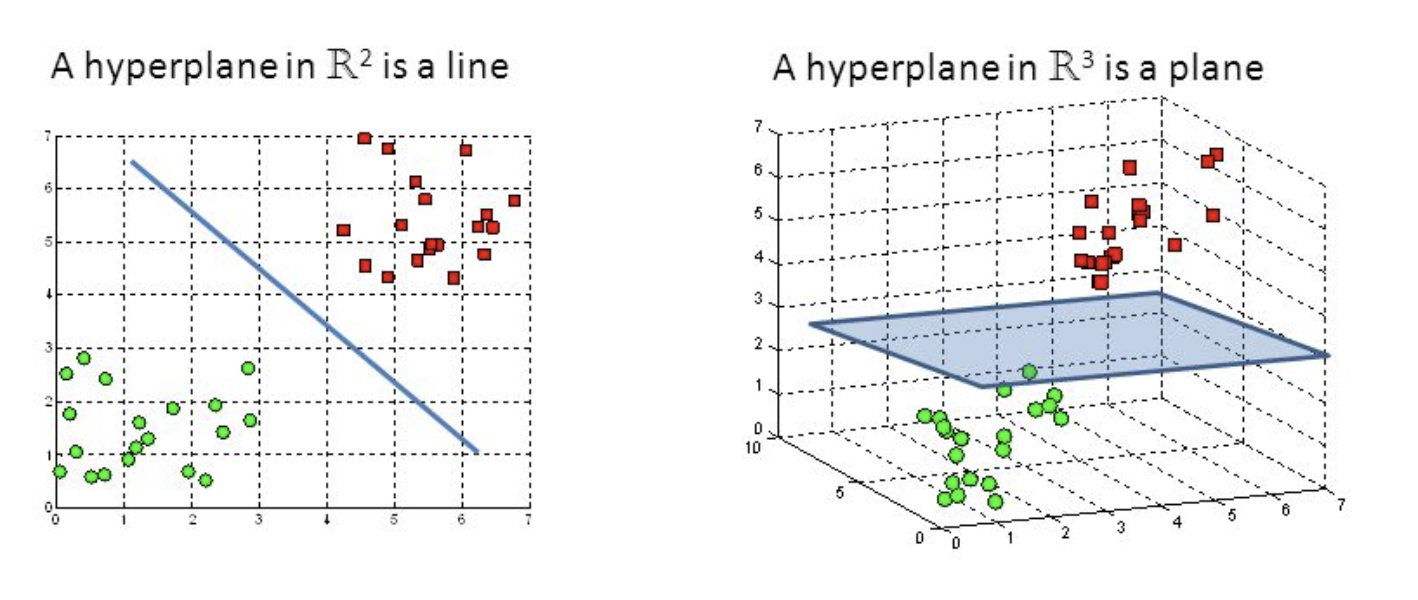
\includegraphics[width=0.7\linewidth]{graphs/hyperplane.png}
    \caption{Illustration of hyperplanes in different dimensions \cite{Hyperplane}}
    \label{fig:hyperplane}
\end{figure}

In artificial neural networks, classification refers to the process of assigning given input values to one of several predefined classes based on specific patterns within the data. A key goal of a classification network is to find a decision boundary that can separate discrete regions corresponding to each class. ANNs find decision boundaries through an iterative process of training and adjusting the weights and biases accordingly to minimize classification error by using backpropagation. After the training phase, the network uses the learned decision boundary to classify unseen data points. The classification process can be broken down into three main steps: first, the input data is passed through the input layer, where each neuron represents a feature of the data. Next, the network processes the data through the hidden layers, where relevant features are extracted using weighted sums, biases, and activation functions. Finally, the processed data reaches the output layer, where the network assigns a class based on the neuron with the highest output value, providing the network's ultimate prediction.

To achieve the correct class assignment, the network tries to find a hyperplane, a line in a two-dimensional space or a plane in higher dimensions, that best separates the data points into distinct classes (illustrated in Figure \ref{fig:hyperplane}). The decision boundary is typically a mathematical function in which the input features are weighted, summed, and passed through an activation function. If the output exceeds a certain threshold, the data point is classified as one class; otherwise, it is classified into another.

However, when the data is not linearly separable, meaning a single straight line cannot separate the classes, the network uses multiple layers to create more complex non-linear decision boundaries. These non-linear boundaries are formed by stacking hidden layers and applying non-linear activation functions. Each layer learns progressively higher-level features of the data, allowing the network to model more complex patterns and therefore make more accurate decisions in classification tasks.

\section{Methodology}
In this section, we describe our approach to implementing dynamic target value optimization for neural network classification. First, we break down the concrete architecture of the target vectors used for training and classification. Then we describe two algorithms which will be used to generate and dynamically adjust these target vectors.

\subsection{Target Value Architecture}\label{sec:targets}

To establish our methodology clearly, it is important to note that in this work, a \textit{class} is represented not by a single neuron but by a full target vector that encodes the network's idealized response to inputs from that class. This contrasts with the traditional view, where each class is tied to a unique output neuron. With this in mind, we first review the standard one-hot encoding approach before introducing our alternative target value structure.

In standard classification with $C$ classes, the target vector $\mathbf{t}^{(i)}$ for a sample belonging to class $i$ is defined as:

$$\mathbf{t}^{(i)} = [0, 0, \ldots, 0, \underbrace{1}_{i\text{-th position}}, 0, \ldots, 0]$$

For example, with 3 classes, the target vectors are:
$$\mathbf{t}^{(1)} = \begin{bmatrix} 1 \\ 0 \\ 0 \end{bmatrix}, \quad 
\mathbf{t}^{(2)} = \begin{bmatrix} 0 \\ 1 \\ 0 \end{bmatrix}, \quad 
\mathbf{t}^{(3)} = \begin{bmatrix} 0 \\ 0 \\ 1 \end{bmatrix}$$
As discussed in Section~\ref{sec:class}, these vectors represent the desired outputs of the network for each class. For instance, when the input belongs to class 1, the first output neuron should produce 1 while the others should produce 0. The more the actual output deviates from this target, the higher the loss will be, and the more the network will need to adjust.\\ 

As such, the target vectors specify what the output neurons should produce, and comparing these targets to the network's actual outputs yields the loss.  The method by which we construct these target vectors is, however,  not set in stone, it is a design choice. The real question is whether a particular method proves effective for learning.

\subsection{Class and Non-Class Values}\label{sec:candnc}
A simple approach to constructing these target vectors is the one-hot method discussed in the previous subsection. Here we aim to define a more abstract way of looking at this and other similar methods of target vector construction. 

Let us first lay out two ways of thinking about how the one-hot method constructs its target vectors: 
\begin{enumerate}
\item \textbf{Class-focused view:} Each class is assigned a neuron and two values (for one-hot these are always 1 and 0). To construct the target vector for a sample, we identify its class and set the entry corresponding to that class's neuron to 1, while all other entries are set to 0.

\item \textbf{Position-focused view:} Each class is still assigned a neuron and two values, but now we build the vector by inspecting each position in turn. For every entry we ask: does this position correspond to the neuron of the current class? If yes, assign it the first value of this class (here 1); if not, assign it the second value associated with \textit{the class of that neuron} (here 0).

\end{enumerate}

These two ideas perform the same when applied to one-hot encoding since every class uses the same two values of 0 and 1, but they are not identical. Using distinct values for different classes would result in these two views producing differing target vectors for the same chosen values. Our method of choosing and dynamically updating target values is based entirely on the first (class-focused) view, we mention the second view here because it will play a role in Section~\ref{sec:disc}.\\

With this background, we can easily define our method for constructing target vectors. Before ever constructing a target vector, we go through the following steps:
\begin{enumerate}
    \item  Go through all classes and assign a unique output neuron to each one.
    \item For each class, define the value that will occupy the position in the target vector corresponding to its assigned output neuron. We will refer to this value as the \textit{class value} of that class, denoted $c_{i}$ for class $i$. 
    \item For each class, define the value that will occupy all other positions in the target vector, namely those that do not correspond to its assigned output neuron. We will refer to this value as the \textit{non-class value} of that class, denoted $\bar{c_{i}}$ for class $i$.
\end{enumerate}

When we now want to construct the target vector for a sample of a particular class, it is as simple as inserting that class's class value into the designated position of the vector (the one corresponding to the assigned neuron) and inserting the non-class value everywhere else. This results in the following target vector for any sample of class $i$:
$$\mathbf{t}^{(i)} = [\bar{c_i}, \bar{c_i}, \ldots, \bar{c_i}, \underbrace{c_i}_{i\text{-th position}}, \bar{c_i}, \ldots, \bar{c_i}]$$
The approach gives us two parameters for each class, which we can freely initialize and alter dynamically during training. In principle, one could assign a distinct non-class value to each of the
$i-1$ remaining positions in the target vector. For simplicity, however, we use a single non-class value $\bar{c_i}$ per class and apply it uniformly to all non-designated positions.

\subsection{Sigma Adaptation Algorithm}\label{sec:sigma}
Now that we have established the class and non-class values, our next step is to find an algorithm that dynamically initializes and adjusts these values according to the network's output tendencies during training. We will then evaluate whether this approach improves the training process and how it compares to traditional methods. The core of this algorithm was first developed by Begic et al. and named the "Sigma Adaptation" algorithm \cite{begic}. In the following, we describe our interpretation of an extended version of this algorithm proposed by Almasov-Misaev et al. \cite{almasov}.

The algorithm consists of four components: \textit{pretraining},  \textit{profiling}, \textit{spacing}, and \textit{correction}. In the pretraining step, we calculate the initial class and non-class values. Profiling records statistics about the target values and network outputs during training. Spacing uses these statistics to adjust the class and non-class values. Finally, the correction step ensures that the adjusted values respect the necessary constraints. The following subsections describe each component in detail.

\subsubsection{Pretraining}
Before training begins, we assign each output neuron to a class as discussed in Section~\ref{sec:candnc}. To initialize the class and non-class values, we run a forward-only pass over the dataset without updating the weights and record the output activations for each sample. The class value $c_i$ is computed by averaging the activations of the assigned output neuron across all samples of class $i$. The non-class value $\bar{c}_i$ is obtained in the same way, but averaged across all non-assigned neurons. With these initial values determined for each class, training can begin. An addition to the algorithm as compared to the Almasov-Misaev et al. version is an optional nudge which can be applied to the non-class values $\bar{c_i}$, moving them away from their corresponding class values $c_i$. The amount by which the non-class value is moved can be freely chosen. We also ensure that it does not go out of bounds by applying the correction described in Section~\ref{sec:correct}.

\subsubsection{Profiling}
During every epoch in training, we collect several values for each class. Whenever a sample is forwarded through the network, we store the activation of the output neuron assigned to that class in a list of that class's "class value predictions." The activations of the other output neurons are stored in a list of this class's "non-class value predictions." At the end of the epoch, we calculate the standard deviation of all class value predictions ($\sigma_i$) and all non-class value predictions ($\bar{\sigma_i}$). We then take the sum of these two standard deviations, which leaves us with $\sigma^{sum}_i$ for each class $i$.

\subsubsection{Spacing}\label{sec:spacing}
The goal of spacing is to enforce a minimum separation between class and non-class values. To that end, we compute the distance between each class value $c_i$ and its corresponding non-class value $\bar{c}_i$ and ensure the distance between them is at least $\sigma^{\text{sum}}_i$. If the distance is smaller than this threshold, $\bar{c}_i$ is adjusted as follows:

\begin{itemize}
    \item \textbf{Case 1:} If $\bar{c}_i > c_i$, then $\bar{c}_i$ is pushed upward by $\sigma^{\text{sum}}_i$.
    \item \textbf{Case 2:} If $\bar{c}_i \leq c_i$, then $\bar{c}_i$ is pushed downward by $\sigma^{\text{sum}}_i$.
\end{itemize}

\subsubsection{Correction}\label{sec:correct}
Depending on the activation function used, the range of values the output neurons can produce may be restricted. For example, a sigmoid activation function constrains outputs to the interval $[0,1]$. If during spacing the non-class value $\bar{c}_i$ is pushed outside this valid range, we clamp $\bar{c}_i$ to the nearest boundary $b \in \{0,1\}$ and set the class value to
\[
c_i = b \pm \sigma^{\text{sum}}_i,
\]
where the sign is chosen to ensure that $c_i$ remains within bounds and separated from $\bar{c}_i$ by at least $\sigma^{\text{sum}}_i$.

\subsection{Base Algorithm}\label{sec:base}
In addition to the Sigma Adaptation Algorithm described in Section~\ref{sec:sigma}, we introduce a stripped-down \textit{Base Algorithm} that omits the spacing step during training. We include this baseline because the spacing step lacks a theoretical justification, having been adopted from the prior group's algorithm largely on intuitive grounds. This makes it important to evaluate whether a similar algorithm without spacing performs better or worse.

\section{Experimental Setup}
 Our experimental setup is designed to evaluate the performance of our dynamic target value optimization method against traditional one-hot encoding and soft-target baselines. All experiments are conducted on the MNIST dataset.

 \subsection{Network Architecture}\label{sec:net_arch}
All experiments use convolutional neural  networks (CNNs) , implemented in PyTorch.

 \begin{itemize}
     \item An initial convolutional layer with 1 input channel, 10 output channels, and a kernel size of 5.
     \item A second convolutional layer with 10 input channels, 20 output channels, and a kernel size of 5. A dropout layer is applied after this convolution.
     \item A fully connected layer with 320 input features and 50 output features.
     \item A final fully connected layer with 50 input features and 10 output features, corresponding to the 10 digit classes.
 \end{itemize}
 The network uses sigmoid activation functions after the convolutional and first fully connected layers and a log softmax activation function on the output layer.

 \subsection{Training Parameters}
 The training process is configured with the following hyperparameters:
 \begin{itemize}
     \item \textbf{Epochs:} The number of training epochs is configurable but typically set to 4 for our experiments.
     \item \textbf{Batch Size:} We use a batch size of 64 for training and 1000 for testing.
     \item \textbf{Optimizer:} Stochastic Gradient Descent (SGD) is used as the optimizer, with a learning rate of 0.01 and momentum of 0.5.
     \item \textbf{Loss Function:} The loss is calculated using the negative log likelihood loss (NLL) between the network's log softmax output and the target vectors.
 \end{itemize}

 \subsection{Target Value Strategies}
 We compare four different target value strategies:
 \begin{enumerate}
     \item \textbf{One-Hot Encoding:} The traditional approach, where the target vector for the correct class contains a 1 at the corresponding index and 0s elsewhere.
     \item \textbf{Soft Targets:} A variation where the target for the correct class is set to 0.8 and the targets for all other classes are set to 0.2.
     \item \textbf{Sigma Adaptation:} The method of producing target vectors described in Section~\ref{sec:sigma} \cite{begic}.
     \item \textbf{Base Algorithm:} Our stripped-down version of the Sigma Adaptation algorithm, described in Section~\ref{sec:base}.
 \end{enumerate}

 \subsection{Evaluation Metrics}
 The performance of each strategy is evaluated based on the following metrics, which are logged using Weights \& Biases:
 \begin{itemize}
     \item \textbf{Hard Accuracy:} Hard accuracy is defined as the percentage of correctly classified images. For standard one-hot targets, the predicted class is the output neuron with the highest activation. However, with Sigma Adaptation and the Base algorithm, this rule no longer applies. Instead, we treat the networks output as a vector and compute its Euclidean distance to each \textit{class's target vector} (see Section~\ref{sec:targets}.) The predicted class is taken to be the one whose target vector is closest to the output vector.
     \item \textbf{Test Loss:} The average NLL on the test set.
     \item \textbf{Confidence:} The average cosine similarity between the network's output and the target vector of the predicted class.
     \item \textbf{Target Value Separation:} For the dynamic target method, we track the absolute difference between the class and non-class target values for each class, as well as the average, minimum, and maximum separation across all classes.
 \end{itemize}

\section{Results}
In this section, we examine how the proposed methods perform in practice and how they compare to traditional methods like one-hot encoding and soft targets.

\subsection{Performance Comparison}
To compare the performance of these approaches, we examine accuracy over training time, focusing on both final performance and convergence speed.
\begin{figure}
    \centering
    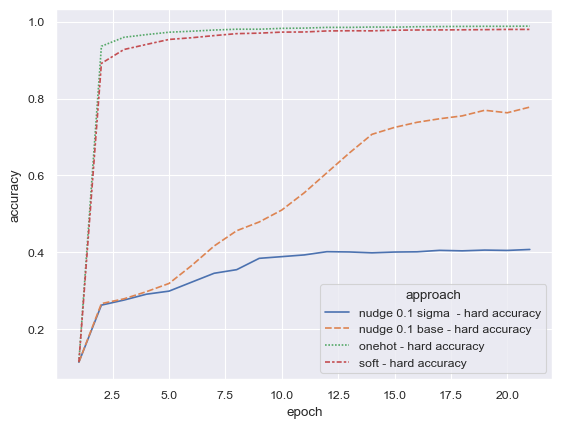
\includegraphics[width=0.6\linewidth]{graphs/acc.png}
    \caption{Accuracy Over Time}
    \label{fig:acc}
\end{figure}

As shown in Figure~\ref{fig:acc}, the one-hot and soft target approaches achieve over 90\% accuracy within the first 3 epochs. In contrast, the model using the Base algorithm reaches just under 80\% accuracy after 20 epochs, while the variant using the Sigma Adaptation algorithm plateaus at approximately 40\% accuracy by epoch 10.

\subsection{Accuracy and Confidence}
In Table~\ref{tab:accuracy_confidence}, we compare the final accuracy and confidence of the four different approaches after training for 20 epochs.
\begin{table}[h!]
\centering
\caption{Hard accuracy and confidence of different approaches.}
\begin{tabular}{lcc}
\hline
\textbf{Approach} & \textbf{Hard Accuracy} & \textbf{Confidence} \\
\hline
One-Hot Encoding   & 1.00 & 0.99 \\
Soft Targets       & 0.98 & 0.70 \\
Nudge 0.1 Base     & 0.78 & 0.98 \\
Nudge 0.1 Sigma    & 0.41 & 0.99 \\
\hline
\end{tabular}
\label{tab:accuracy_confidence}
\end{table}

While accuracy varies dramatically across methods ($\sim$ 100\% for soft/one-hot targets, 78\% for Base algorithm, 41\% for Sigma Adaptation), confidence remains consistently high ($\sim$ 100\%) for all approaches except soft targets. This creates a stark mismatch between confidence and actual performance for the dynamic target value methods.

\subsection{Loss Development During Training}
Figure~\ref{fig:loss} shows the development of training loss over the 20 epochs for all four approaches, as well as a magnified view of just the Base and Sigma Adaptation approaches.

\begin{figure}[H]
\centering
\subfigure[Loss development over training epochs\label{fig:all_loss}]{%
    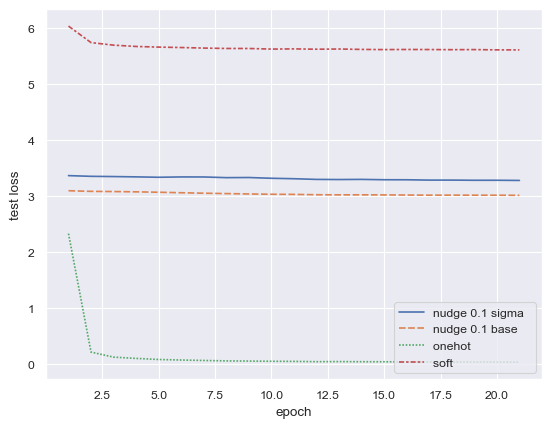
\includegraphics[width=0.48\textwidth]{graphs/loss.png}
}
\hfill
\subfigure[Loss development of base and sigma approaches\label{fig:dyn_loss}]{%
    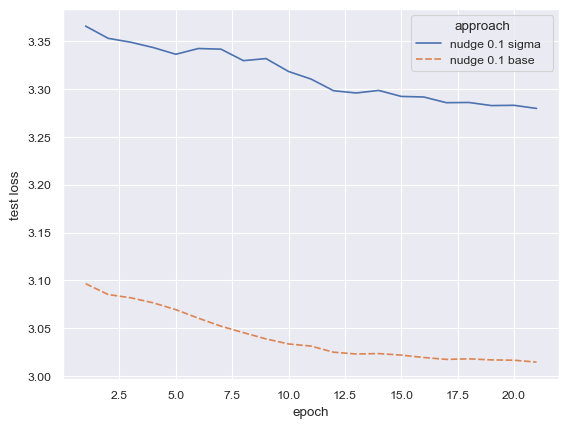
\includegraphics[width=0.48\textwidth]{graphs/lossdyn.png}
}
\caption{Training loss comparison across different target value strategies}
\label{fig:loss}
\end{figure}

The test loss of the one-hot and soft target approaches develop in line with their accuracy, showing a steep drop-off in the first few epochs, then slowly decreasing until the end of training. The loss in the dynamic target approaches decreases steadily throughout the entire training, without speeding up or slowing down significantly at any point.

\subsection{Accuracy and Target Value Separation}
In Figure~\ref{fig:accvsep} we compare the development of accuracy with the average distance between class and non-class values in between both dynamic target value approaches.

\begin{figure}[H]
    \centering
    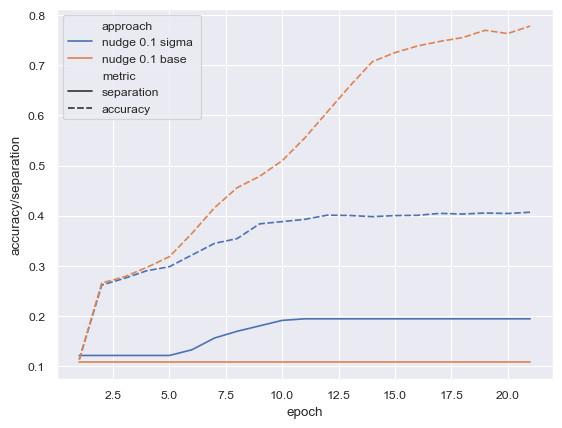
\includegraphics[width=0.6\linewidth]{graphs/accvsep.png}
    \caption{Accuracy vs. Target Value Separation}
    \label{fig:accvsep}
\end{figure}

While the Sigma Adaptation approach gradually increases its average separation between epochs 5 and 10, the Base approach maintains a constant separation between the class and non-class values throughout training. The Sigma Adaptation approach enhances its accuracy only during the initial two epochs and during the separation change, while the non-spaced Base approach experiences an overall increase in accuracy throughout the training process.

\subsection{Target Values Over Time}
The following is an example of how the target values are initialized and how they develop over time.
\begin{figure}[H]
    \centering
    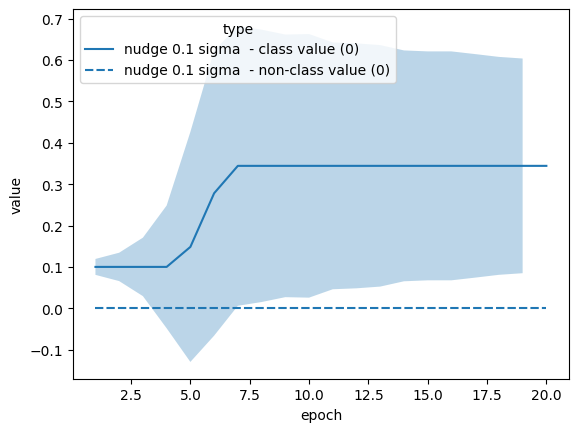
\includegraphics[width=0.5\linewidth]{graphs/sigma.png}
    \caption{Class and non-class value development over 20 epochs}
    \label{fig:class_dev}
\end{figure}

In Figure~\ref{fig:class_dev} see the class value (full) and non-class value (dotted) for class 0 in the MNIST dataset over the course of training the CNN. The blue area represents $\sigma^{sum}_0$, or rather, the area within a distance of $\sigma^{sum}_0$ from the class value. 

The class and non-class values are likely initialized to around $0.1$ and $0$ respectively during pretraining. The nudge value $\epsilon = 0.1$ suggests that both were near $0$ when initially generated and then nudged apart to their positions at the beginning of the graph.\\

We also observe that, as described in Section~\ref{sec:sigma}, when the non-class value comes within a distance of $\sigma^{sum}_0$ to the class value, we attempt to move the non-class value down. Since the non-class value is already at the lower bound of $0$ here, the class value is moved up by $\sigma^{sum}_0$ instead.


\section{Discussion and Potential Next Steps}\label{sec:disc}
The aim of this section is to analyze the results of our experiments and find potential explanations for the observed behavior, as well as to point out any meaningful correlations in the data.

\subsection{Interpreting the Results}
In this section, we analyze the outcomes of our experiments, discuss their implications, and propose possible explanations for the observed behaviors.


\subsubsection{Performance Analysis: The Confidence-Accuracy Mismatch}
The core insight which can be gained from these experiments is that these novel approaches are, in their current form, not suitable for practical applications. The initial goal was to achieve better training speed or reduce overfitting while maintaining useful accuracy. However, our results demonstrate that the proposed dynamic target methods deliver neither benefit: they achieve significantly lower accuracy (40-80\%) compared to traditional methods ($> 90\%$), while paradoxically maintaining high confidence ($\sim 100\%$) that undermines any potential regularization benefits (Table~\ref{tab:accuracy_confidence}).
Where the one-hot approach delivers the best overall accuracy and training speed, the regular soft target approach exhibits similar accuracy with appropriately lower confidence, therefore acting against overfitting. Our dynamic approaches occupy a poor position in this trade-off space (low accuracy combined with overconfident predictions) making them unsuitable for applications where either high performance or well-calibrated uncertainty is required.

\subsubsection{The Divergence Between Loss and Accuracy}
Where Figure~\ref{fig:dyn_loss} clearly shows the loss of the dynamic target approaches decrease steadily during the entire training process, the accuracy (as seen in Figure~\ref{fig:acc}), especially of the Sigma Adaptation approach, does not mirror this trend as might be expected. While the decreasing loss does indicate that the network is learning, it appears that the spacing process of the algorithm (see Section~\ref{sec:spacing}) inhibits the translation of this learning into improved classification accuracy. A potential explanation may be that, while the predictions do overall become more similar to the correct targets, the frequent movement of the class and non-class values prevents this increase in similarity from actually resulting in the closest target vector being the one from the correct class.

While this "moving target" explanation could potentially contribute to the issue, the target values do eventually stabilize around epoch 10 (Figure~\ref{fig:accvsep}). This indicates that there exists some more profound issue with the Sigma Adaptation algorithm as described in Section~\ref{sec:sigma}, which drives class and non-class values into positions which are fundamentally unsuitable for effective classification.

\subsubsection{Target Value Dynamics and Their Impact}
As opposed to the Sigma Adaptation the Base approach (without spacing) exhibits a slightly better accuracy / confidence ratio.

The concept of adapting the labels according to some external factor is not entirely novel, for example in adaptive label smoothing, where the smoothing factor is determined by a property of the input data \cite{krothapalli_adaptive_2020}. Despite this, assigning labels solely based on the untrained network's output is an unexplored field that could use more study. 

\subsubsection{Experiment Complexity}
A key issue with our experiments is the use of a CNN. While CNNs are the industry standard for image classification tasks, testing of a novel concept such as this would be far better served by a simpler architecture that yields more explainable results. As it stands, the reasons for most of our results remain guesswork; this could have been avoided to some extent by using a simpler architecture.

\subsection{Future Work}
There are a number of possible next steps that could be helpful in further exploring the potential of approaches akin to the ones described here. We believe the main issue with our approach lies not in the concept itself but in a design decision made early in our process. In Section~\ref{sec:candnc} we describe two high-level approaches for constructing target vectors: the class-focused view and the position-focused view. While we settled on the class-focused view due to its perceived simplicity, we did not consider the effect this would have on the generated target vectors, and indeed on the network itself, in enough depth.\\

Under the class-focused view, each class's target vector seems simple, it consists only of the class value and the associated non-class values. However, this design means that each output neuron (corresponding to a position in the target vector) is trained not toward just two values, but toward $i$ values, where $i$ is the number of classes. Each neuron must therefore take on its assigned class's value as well as $i-1$ different non-class values, one for each other class. This may introduce instability during training and confuse the network. For this reason, it would be valuable for future work to examine how the Sigma Adaptation algorithm performs when applied under the position-focused view of target vector construction.


\section{Summary and Conclusion}
In this project, we explored an alternative method to one-hot encoding for initializing target values in neural network classification tasks by assigning custom target values that depend on the models' untrained outputs and dynamically evolving them throughout training.

Our main findings included an overall lack of viable performance across both our approaches when compared to traditional methods. Here the main challenges were fundamental design decisions and an overly complex experiment setup.\\

The idea of capturing the network's preferences remains interesting. While some parts of our approach seem to fall just short of being useful, other parts require more careful reconsideration. Future works could focus on applying the described Sigma Adaptation algorithm under different assumptions about target vector construction or about how to extract the "preferences" of the neural network in the first place.

% real scientific references
\bibliographystyle{ieeetr}
\bibliography{references}		% .bib files here

\end{document}